\documentclass[12pt, a5paper, twoside]{book}

\usepackage{float} % incluir imagens
\usepackage[export]{adjustbox} % centralizar
\usepackage{subcaption} % legendas
\usepackage{graphicx}
\graphicspath{ {pic/} }

\usepackage[pass]{geometry}

\usepackage{setspace}
\onehalfspacing{}

\usepackage{indentfirst}
\usepackage[skip=0pt, indent=1.25cm]{parskip}

\usepackage{ragged2e}
\justifying{}

\usepackage[portuguese]{babel}
\usepackage{hyphsubst}

\usepackage{fontspec}

\newenvironment{dedication}{
    \clearpage
    \thispagestyle{empty}
    \vspace*{\stretch{3}}
    \small
    \itshape
    \raggedright
}{\par\vspace*{\stretch{1}}\clearpage\normalfont} % taken from https://tex.stackexchange.com/questions/476646/how-put-title-in-a-dedication

\title{História da Família, Parte II}
\author{Teresa Cristina}
\date{2025}

\renewcommand{\thechapter}{\Roman{chapter}}

\begin{document}

\begin{titlepage}
\maketitle 
\end{titlepage}

\begin{dedication}
Aos meus filhos, para que, tal como ensinou Terêncio, nada que seja humano, lhes seja estranho. 
Aos que cobrarem maior fidelidade aos fatos, saibam que o que aqui vai contado, vai tal e qual a emoção esculpiu na alma e a memória arquivou sem contestar. 
Pois nunca sabemos com exatidão o que de fato acontece. 
O que fica é o que nos parece e como nos parece no momento do acontecido. 
\end{dedication}

\tableofcontents

\chapter{}
Sou do tempo bom em que os adultos se livravam das crianças sem culpa, mandando: ``Vão brincar lá fora!''.
E ``lá fora'' era o quintal, o maravilhoso país da infância.
Sobretudo quando se vivia numa cidade do interior. 
Era o espaço de descobrir e pensar o mundo. 
Observar as formigas na sua labuta incessante, as lagartixas subindo pelo velho muro meio rachado, as borboletas iridescentes, o rastro prateado e gosmento desenhado pelos vagarosos caracóis.   
Contemplar a incessante migração das nuvens que o vento ora esfiapava, ora ia juntando em formas caprichosas de bichos, árvores, gigantes, castelos, anjos e às vezes mapas, como aqueles pendurados nas paredes da sala de aula. 
Sentir o cheiro da roupa lavada e embebida de sol, pendurada no varal; da fumaça desprendendo-se da lenha queimada no fogão; da terra molhada, da moita de arruda, das rosas, do jasmim, do manacá; do bafio úmido de sepulcro que emanava da escura caverna do porão. 
Deitada de costas nas pedras quentes da calçada, abandonava-me ao sol. O calor invadia aos poucos meu corpo, amolecendo braços e pernas e eu os imaginava penetrando terra adentro, como raízes. 
Imóvel, escutava o zunido das abelhas nas flores, os recados insistentes do ``fogo apagou'' e do bem-te-vi vindos lá das bandas do cemitério, o canto dos sabiás e a algazarra dos pardais e andorinhas sobrevoando a velha paineira do almoxarifado da prefeitura bem ali, do outro lado da rua. 
Na marcenaria, alguns quarteirões acima, o som plangente da serra cortando madeira dividia com o sino da torre da Matriz a tarefa de marcar regularmente a passagem das horas. 
Vez ou outra, roncando em agonia a cada mudança de marcha, os velhos ônibus a querosene passavam sacolejando nos paralelepípedos, rua acima; os carros ainda eram raros. 
E, do outro lado do muro, do barracão da fábrica do meu pai, chegava o som oceânico, abafado e constante das máquinas torcendo os fios de algodão para transformá-los nos novelos de barbante que garantiam o sustento da nossa família e a minha doce vadiagem de criança.

As cores, formas e textura das flores e folhagens me fascinavam. 
Recobriam meus desenhos infantis e emolduravam em cercaduras delirantes as páginas dos meus cadernos de escola.

Na opinião da minha mãe, as flores do nosso quintal deviam obedecer à moda, como tudo o mais. 
Lembro-me da fase dos crisântemos, dálias e crisandálias repolhudas, logo repudiadas em favor das rosas que, por sua vez, acabaram arrancadas para dar lugar às palmas de Santa Rita e às gérberas. 
Essas mudanças eram quase sempre decididas por volta do Dia de Finados, quando as parentes da Capital chegavam sobraçando as novidades compradas nas floriculturas do Arouche. 
Houve uma vez em que a matriarca das hostes paulistanas, Tia Angelina, desceu do trem exibindo buquês de soberbos e inacreditáveis gladíolos azuis. Foi o quanto bastou para que as nossas pobres palmas de Santa Rita caíssem em desgraça. 
``Coisa mais calú!'', decretou minha mãe. 
Era sua expressão favorita para o que lhe parecia vulgar ou caipira. O projeto do novo jardim teve, porém, que ser adiado. 
De tanto mexer na terra, nas sucessivas reformas dos nossos canteiros, mamãe arrumou uma infecção persistente nos dedos que acabou por lhe fazer caírem as unhas. 
Até um médico especialista em São Paulo precisou ser consultado, já que o nosso habitual curandeiro, o Joãozinho da Farmácia, amigo de longa data do papai, não conseguiu resolver a tal eczema.

De qualquer modo, outros e mais amplos planos de mudança começavam a agitar minha família, pois mamãe começara a achar ``calús'' não só as flores, como todo o quintal, a casa antiga de ``parede a meia'' e banheiro fora, os móveis escuros, ``art-déco''. 
Papai prosperava nos negócios e mamãe já podia sonhar mais alto: uma casa moderna, com mais cômodos, armários embutidos, num bairro novo e mais nobre. 
Prenunciando a nova fase, nossa antiga sala de jantar desapareceu para dar lugar a uma mobília nova e aromática, de jacarandá torneado, em que se destacava uma vistosa cristaleira apropriadamente recheada com copos de cristal recém-adquiridos e que tilintavam perigosamente a cada passo nosso sobre o velho assoalho. 
Nossas caminhas \textit{Patente} foram substituídas por outras, artisticamente torneadas também e os velhos colchões de crina foram para o lixo. 
Passamos a dormir em modernos colchões de mola. Um tapeceiro alemão veio tirar as medidas para fabricar sofá, poltrona e cortinas para a sala de estar. 
Coroando todo esse luxo, um dia desembarcou em nosso portão a peça central da nova decoração: um piano de nogueira, novo em folha, que se converteria num dos grandes instrumentos de tortura da minha juventude. 
Porque então, junto com o quintal e a velha casa, ficava para trás também a minha infância. 
Eu me tornara uma adolescente e, em breve, nós mudaríamos para a casa da Av. D. Pedro II, n.º 1273, defronte ao Clube de Campo do Araraquarense. Corria o ano de 1958.

\begin{figure}[H]
\centering
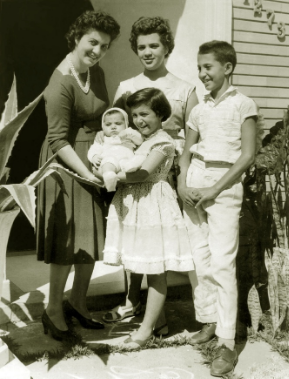
\includegraphics[width=0.5\linewidth]{1/maria-joão.png}
\caption{A família na porta da casa nova. No colo da
Maria Lúcia, o recém-chegado João.}
\end{figure}
\chapter{}
Para o bem e para o mal, minha infância transcorreu numa pequena galáxia de clãs interligados, de origem imigrante e pobre, dos quais os mais importantes eram os Filpi, os Credidio e os Ópice, todos com raízes na Itália. 
Dezenas de olhos e bocas para censurar e orientar e montes de braços para acarinhar e acolher, e uma intensa experiência humana para vivenciar, recolher, degustar e aprender. 

Nossa antiga sala de jantar exibia uma mesa particularmente desgraciosa, quadradona e pesada, mas que, para mim, tinha um encanto especial: embutia um pequeno armário no seu único e largo pé central, onde eram guardados os jornais velhos. 
Um dia descobri que eu cabia direitinho naquele esconderijo e ali, insuspeitada, colhi minhas primeiras e fortes impressões do mundo adulto.  
Era à volta daquela mesa que as visitas se reuniam para o café. 
Era divertido acompanhar, debaixo dela, o movimento das pernas inchadas e nodosas de varizes das tias-avós, na excitação de comentar os acontecimentos da cidade e a vida alheia. 
Quando mamãe e suas irmãs aparteavam a discussão, vez ou outra, contrapondo argumentos mais modernos, arejados por visões do pós-guerra de liberação feminina, difundidas pelo cinema norte-americano quase sempre, as vozes se alteravam, os pés se agitavam e, na ânsia de vencer a contenda, de algum ponto da mesa vinha a cartada definitiva, o disse-me-disse mais recente e irretorquível, quase sempre sussurrado, inalcançável à minha parca compreensão de criança, mas emoldurado pela aura sagrada e misteriosa do interdito\dots 
Um \textit{``oooohhhh!''} seguido de horrorizado silêncio parecia encerrar a conversa. 
Que logo, porém, renascia animada, como fogo sob as cinzas, sempre sublinhada embaixo da mesa pelo entusiasmado balé de pernas e pés. 
Lembro, com nitidez, de uma tarde em que, andando com minha mãe pela rua, ouvi-a chamar a atenção de uma amiga para uma célebre senhora, personagem recorrente nas reuniões à volta da tal mesa, pelo que me lembro, pelas audaciosas e repetidas incursões fora da sagrada cidadela do casamento. 
Olhei na direção indicada e vi uma mulher vestida de preto, grave e majestosa, na penumbra do banco traseiro de um carro escuro e grande.
Divisei-lhe as feições, ainda bonitas na maturidade. 
Séria, ela devolveu o meu olhar fascinado. E o que senti, juro, foi pura admiração.

Dos clãs principais, o da minha mãe era o mais pobre. 
Incluía as irmãs da minha avó Didi, seus maridos e filhos. 
Meu avô João já não tinha mais parentes próximos. 
Dele só conheci um primo engraçado, que vez ou outra aparecia e de novo sumia, como um cometa.  
Embora todas fossem casadas, as Credidio, mulheres invariavelmente fortes e batalhadoras, sobrepunham-se aos machos em autoridade. 
Dessa gente me vieram os impulsos de amar a vida, de superar os revezes sem esmorecer, de correr atrás dos sonhos, mas também a preocupação com as aparências alimentada pelo receio permanente de incorrer em vulgaridade e mau-gosto. 
Alimentavam ambições sociais e acreditavam piamente em cultivar as boas relações para vencer as desvantagens da origem humilde.  
No riso e no pranto, eram pau para toda obra. Com a mesma disposição para encarar bailes e velórios, casamentos, batizados e procissões, envolviam-se em tudo com igual disposição de fazer todo o necessário para que tudo saísse perfeito. 
Davam-se a todas essas empreitadas com sincera devoção e autêntico espírito de caridade e solidariedade. Mas, não dispensavam os holofotes e tinham a deliciosa ingenuidade de nem tentar disfarçar o prazer que sentiam com a repercussão favorável.

O clã do meu pai, os Filpi, embora menos pobre na sua origem, na Itália, já conhecia há muito a inconstância dos fados. 
Lá, na pequena Novi Velia, o patriarca Ângelo viu seus bens esvaírem-se no torvelinho das brigas políticas. 
Aqui, seu filho e meu avô Reginaldo, fazendeiro abastado a quem o café proporcionara razoável fortuna, casa confortável na cidade e educação de qualidade para a prole, perdeu quase tudo na crise de 1929 e teve que levar a família de volta ao recomeço duríssimo na Pedra Branca, única fazenda que lhe restou das quatro ou cinco que chegou a possuir. 
Por conta desses reveses, com certeza, dessa gente me veio um realismo prudente, alicerçado na crença de que estamos cá na terra a serviço e não a passeio, na desconfiança de que todo ídolo oculta pés de barro e de que tudo que reluz quase nunca é ouro, além do mau hábito de trabalhar até o limite das forças. 

O reino das mulheres Filpi era o lar. 
Exímias cozinheiras, incansáveis no lavar, passar, esfregar, bordar e tecer, foram condenadas à vida espartana pelo atraso da minha avó Teresa, uma mente forjada pelo rígido código dos antigos costumes mineiros. 
Mulher era para servir ao homem, pai, irmão ou marido e não para bater pernas na rua e perder-se como as moças pintadas, ataviadas e oferecidas que se viam por aí, querendo diploma, frequentando bailes, usando saias curtas, dirigindo e até fumando! Quando minha mãe, professora formada, frequentadora contumaz dos bailes do clube, exibindo impecáveis unhas esmaltadas e envergando trajes e penteado da moda ingressou na família, não fosse o apoio imediato do galante sogro Reginaldo, certamente seria rechaçada como péssimo exemplo. 
E pelo resto da vida, mesmo após a morte da Vó Teresa, a relação da minha mãe com as cunhadas, foi contraditória: Lectícia era o farol que iluminava para elas os difíceis caminhos da inserção social e da modernidade. 
Mas mamãe, por muitos e muitos anos, padeceu da necessidade neurótica de provar que, apesar das unhas feitas e das roupas da moda, era páreo para elas no comando de um fogão, de um ferro de passar e no brilho das panelas. 
Daí por que preparar um almoço para as cunhadas era um feito precedido por dias de insuportável e cômica tensão, mas que valiam pelo gosto insuperável da vitória, quando o molho e a massa se apresentavam indiscutivelmente no ponto certo. 
Por outro lado, as tias, com meu ouvido treinado em escutar conversa de adultos, ouvia-as muitas vezes lamentar o destino do irmão, coitado, condenado a trabalhar para sustentar os luxos ``daquela gastadeira''.

Os Ópice eram oriundos do casamento de duas irmãs da minha avó materna com dois irmãos recém-chegados da Itália e que vieram estabelecer-se em Araraquara: um hábil alfaiate, chamado Bruno e um não menos hábil carpinteiro chamado José. 
Ao que se conta, ambos exibiam como característica principal um certo refinamento de gostos, incomum entre os pobres imigrantes italianos da região e que provavelmente lhes pareceu suficiente para justificar uma postura algo arrogante e prepotente que sempre os distinguiu, tanto quanto os rompantes de temperamento. 
Afora isso, eram muito trabalhadores e competentes. Todos esses traços são ainda bem visíveis na sua descendência. 
O ramo do Tio Bruno, quase todo, enraizou-se em definitivo na cidade e o do Tio José, algum tempo após a morte precoce deste, acabou migrando para a Capital. 
Os filhos do Tio Bruno, que continuaram a viver sob o jugo do pai, jamais amadureceram totalmente e ficaram na minha memória como uma família de gente boa, meio infantilizada e divertida. 
Os órfãos do Tio José, libertos do autoritarismo paterno, com muito mérito e muito trabalho, fizeram carreira e sólida fortuna na capital. 
E foi assim que se transformaram, para toda a gente da minha mãe, na referência suprema do sucesso, do ``savoir faire'', o exemplo a ser seguido, fonte de jurisprudência a ser consultada em qualquer circunstância e para qualquer assunto. 
Eram respeitosamente designados como ``os de São Paulo'' e sempre que vinham em visita aos parentes da província provocavam um alvoroço que, à medida que nós, os mais novos, crescíamos, acabou virando motivo de piadas sempre recebidas como sacrilégio por vovó, mamãe e suas irmãs. 
Já meu pai que, como bom Filpi, nunca foi afeito a idolatrias de qualquer espécie, fechava o tempo e não foram poucas as vezes em que os pobres Ópice acabaram pagando pela admiração incompreensivelmente servil, no entender do marido, que minha mãe devotava às ideias e realizações dos primos.
\end{document}